\documentclass[12pt, a4paper]{article}

\usepackage[hmargin=2.5cm, vmargin=2cm]{geometry}
\usepackage{amsthm, amssymb, mathtools, yhmath, graphicx}
\usepackage{fontspec, type1cm, titlesec, titling, fancyhdr, tabularx}
\usepackage{color}
\usepackage{unicode-math}
\usepackage{float}
\usepackage{hhline}
\usepackage{comment}
\usepackage{siunitx}
\usepackage{csvsimple}
\usepackage{subcaption}

\usepackage[CheckSingle, CJKmath]{xeCJK}
\usepackage{CJKulem}
\usepackage{enumitem}
\usepackage{tikz}
\usepackage[siunitx]{circuitikz}
\usepackage{wrapfig}
%\setCJKmainfont[BoldFont=cwTex Q Hei]{cwTex Q Ming}
%\setCJKsansfont[BoldFont=cwTex Q Hei]{cwTex Q Ming}
%\setCJKmonofont[BoldFont=cwTex Q Hei]{cwTex Q Ming}
\setCJKmainfont[BoldFont=cwTeX Q Hei]{cwTeX Q Ming}

\def\normalsize{\fontsize{12}{18}\selectfont}
\def\large{\fontsize{14}{21}\selectfont}
\def\Large{\fontsize{16}{24}\selectfont}
\def\LARGE{\fontsize{18}{27}\selectfont}
\def\huge{\fontsize{20}{30}\selectfont}

%\titleformat{\section}{\bf\Large}{\arabic{section}}{24pt}{}
%\titleformat{\subsection}{\large}{\arabic{subsection}.}{12pt}{}
%\titlespacing*{\subsection}{0pt}{0pt}{1.5ex}

\parindent=24pt

\DeclarePairedDelimiter{\abs}{\lvert}{\rvert}
\DeclarePairedDelimiter{\norm}{\lVert}{\rVert}
\DeclarePairedDelimiter{\inpd}{\langle}{\rangle}
\DeclarePairedDelimiter{\ceil}{\lceil}{\rceil}
\DeclarePairedDelimiter{\floor}{\lfloor}{\rfloor}

\newcommand{\unit}[1]{\:(\text{#1})}
\newcommand{\df}[1]{\mathop{}\!\mathrm{d^#1}}
\newcommand{\img}{\mathrm{i}}

\title{ \bf {\Huge 電子電路實驗9:二次線路的頻率響應}\\ 實驗結報}
\author{B02901178 江誠敏}

\begin{document}

\maketitle


\section{實驗結果}
由於數據眾多,因此直接以圖表方式呈現。
\subsection{低通}
\begin{figure}[H]
  \centering
  \begin{subfigure}[b]{0.45\textwidth}
    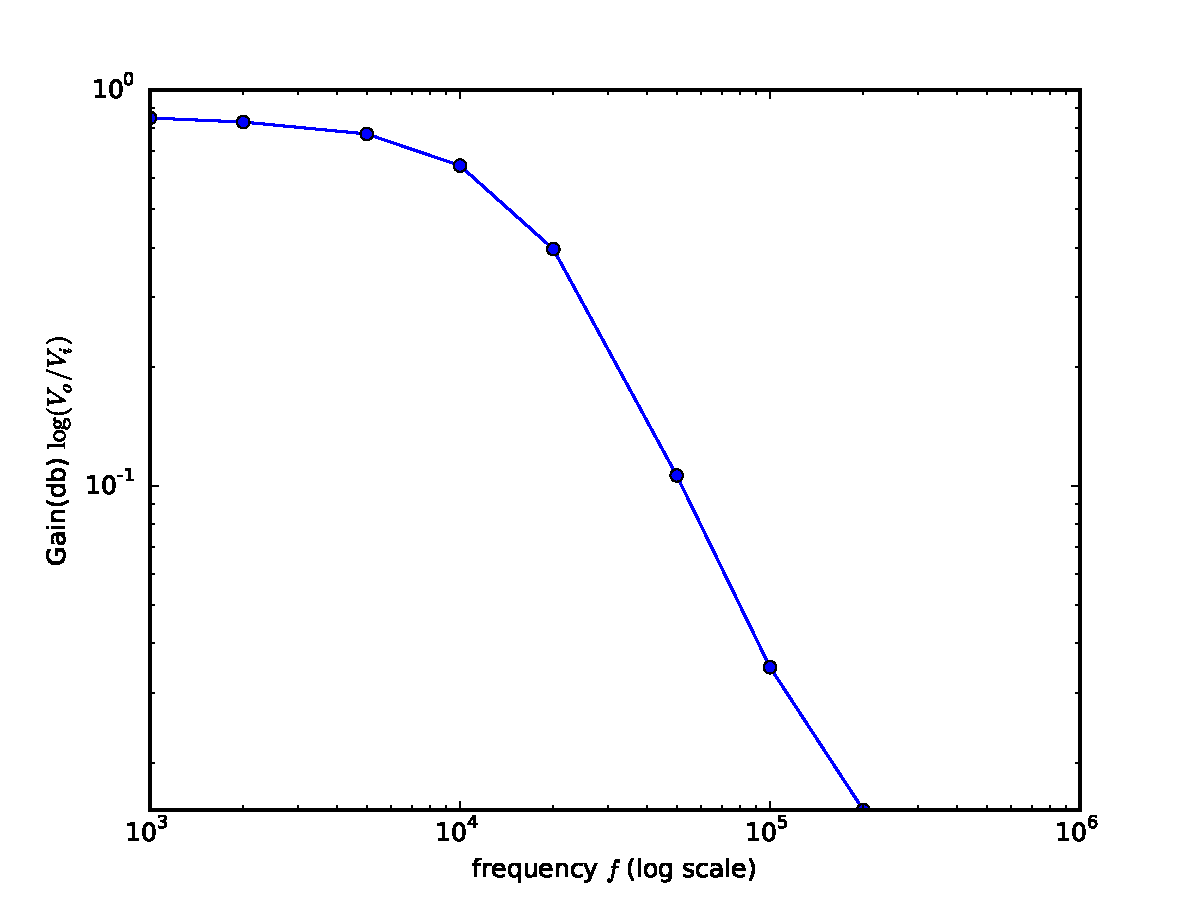
\includegraphics[width=1\textwidth]{data/img/q1.pdf}
    \caption{\SI{510}\ohm}
  \end{subfigure}
  ~
  \begin{subfigure}[b]{0.45\textwidth}
    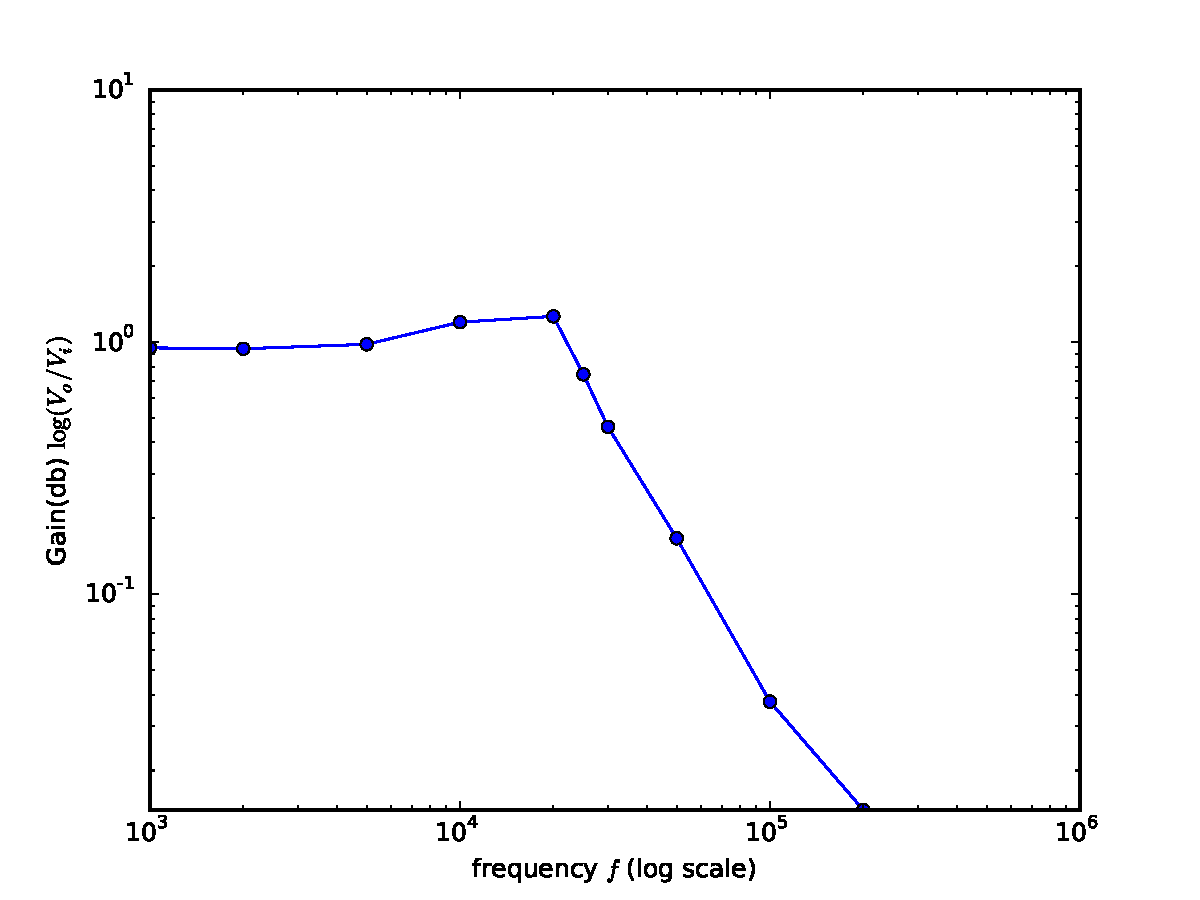
\includegraphics[width=1\textwidth]{data/img/q2.pdf}
    \caption{\SI{2}\kohm}
  \end{subfigure}
\end{figure}

\subsection{高通}
\begin{figure}[H]
  \centering
  \begin{subfigure}[b]{0.45\textwidth}
    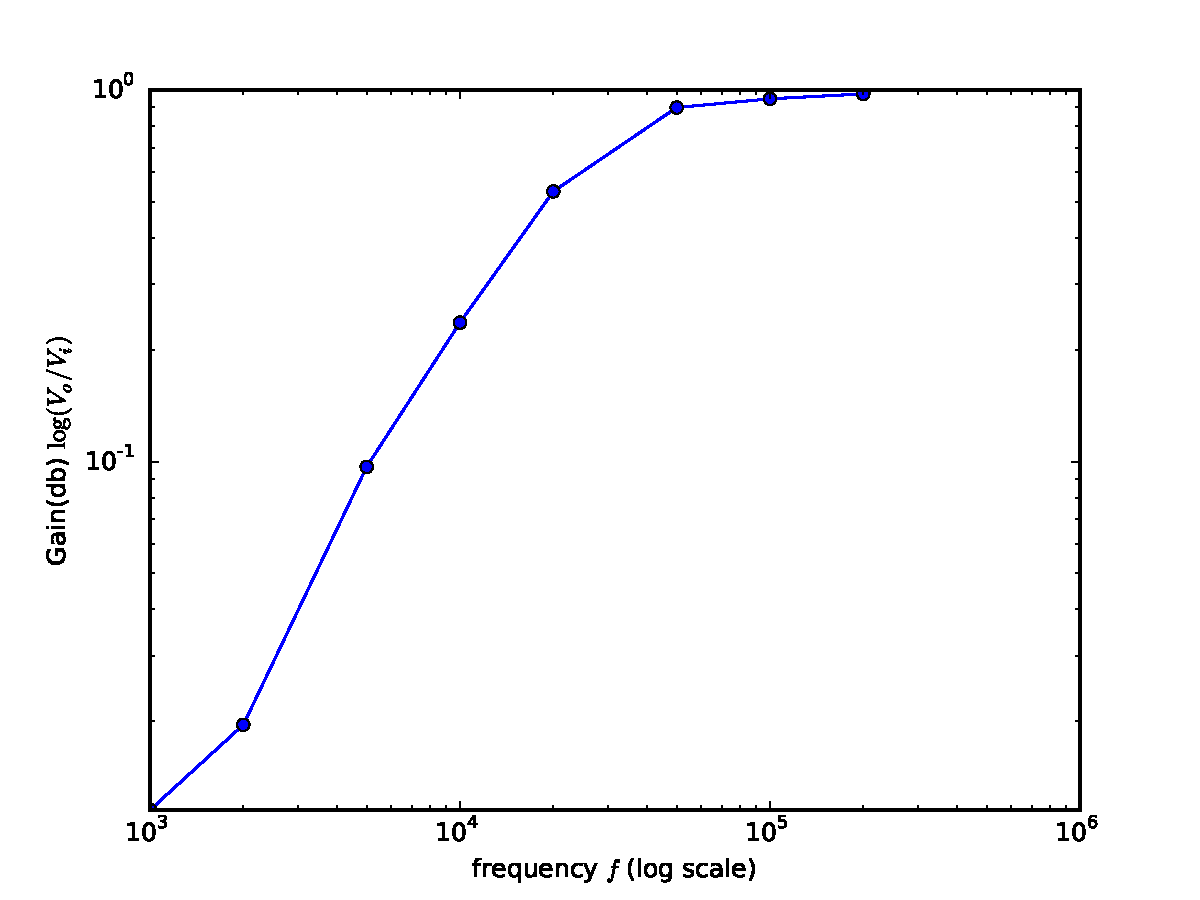
\includegraphics[width=1\textwidth]{data/img/q3.pdf}
    \caption{\SI{510}\ohm}
  \end{subfigure}
  ~
  \begin{subfigure}[b]{0.45\textwidth}
    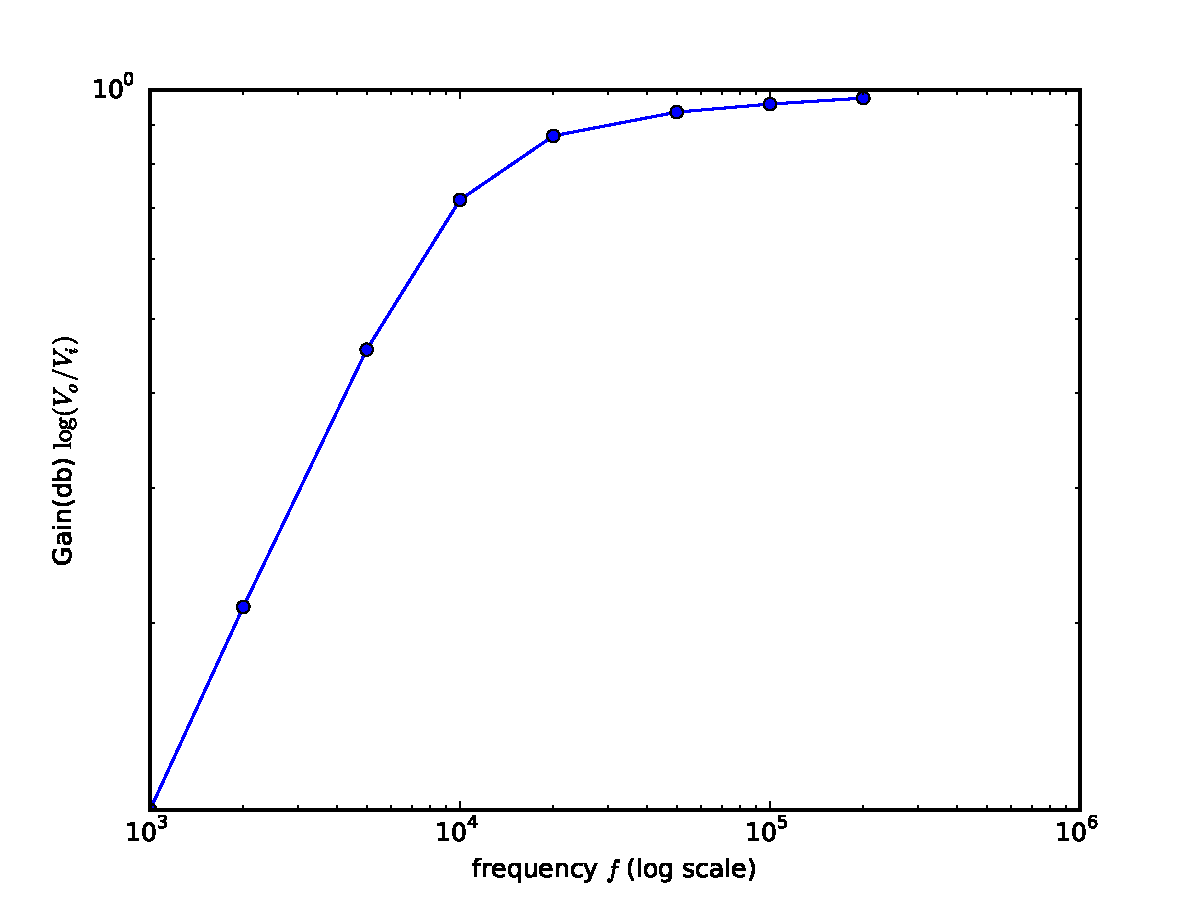
\includegraphics[width=1\textwidth]{data/img/q4.pdf}
    \caption{\SI{2}\kohm}
  \end{subfigure}
\end{figure}
\subsection{帶通}
\begin{figure}[H]
  \centering
  \begin{subfigure}[b]{0.45\textwidth}
    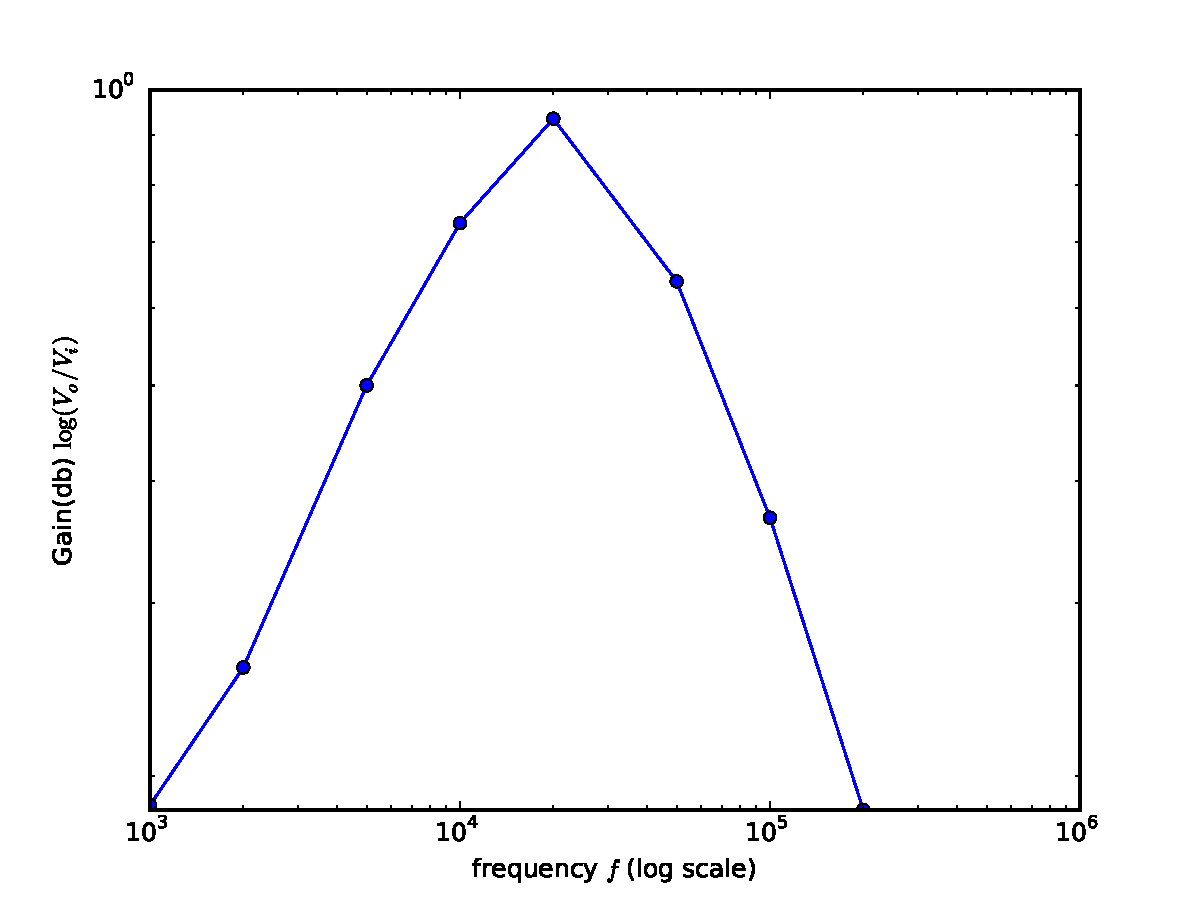
\includegraphics[width=1\textwidth]{data/img/q5.pdf}
    \caption{\SI{510}\ohm}
  \end{subfigure}
  ~
  \begin{subfigure}[b]{0.45\textwidth}
    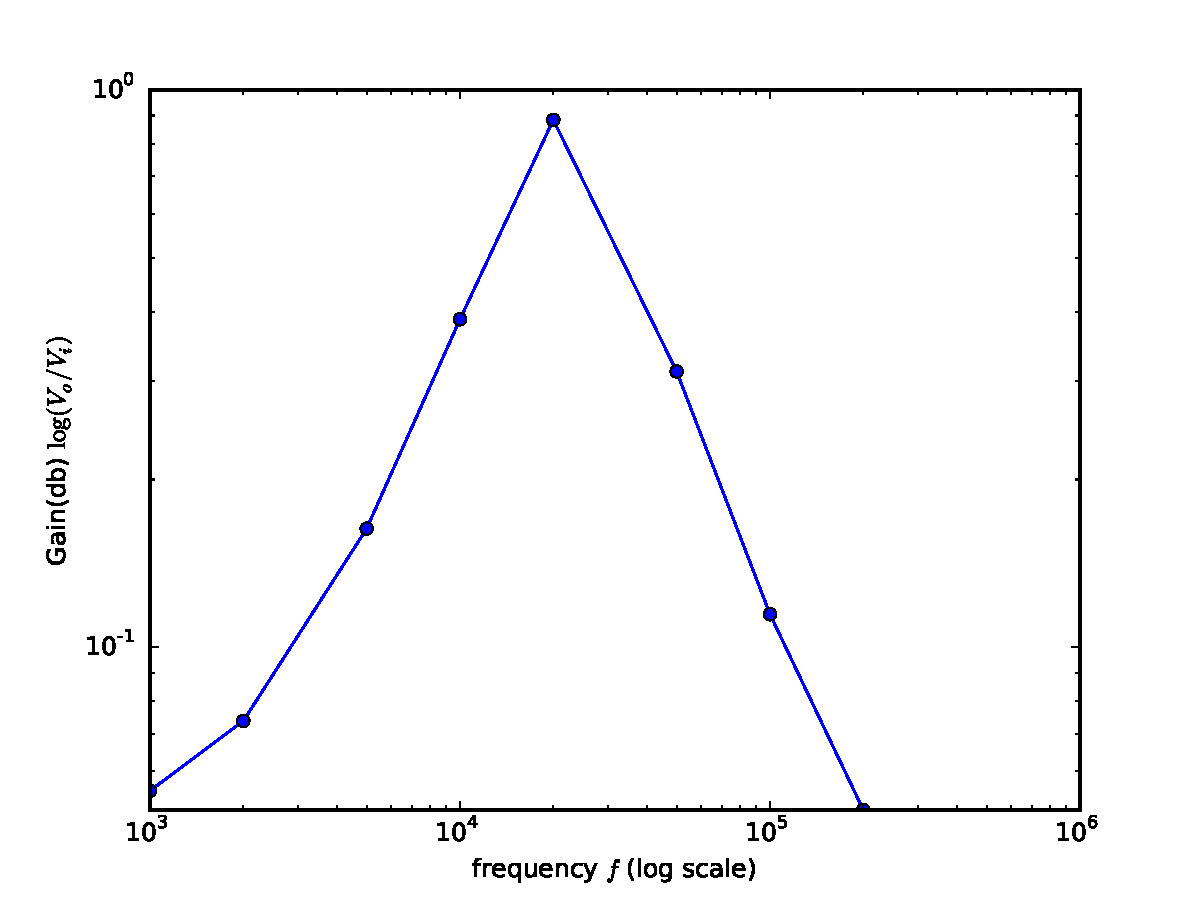
\includegraphics[width=1\textwidth]{data/img/q6.pdf}
    \caption{\SI{2}\kohm}
  \end{subfigure}
\end{figure}




\section{結報問題}

\begin{enumerate}[itemsep=20pt, topsep=10pt]
  \item {\large\bf $R$值的變化對於不同的二次線路的頻率響應有何影響?} \\[10pt]
    答:\\
    \begin{itemize}
      \item 低通、高通:
        我們知道低通、高通的Transfer function分別為
        \begin{align*}
          f(s) &= \frac{R}{R + sL + s^2 LRC} =\frac{1}{1 + (L/R)s + LCs^2} \\
          g(s) &= \frac{s^2 LRC}{R + sL + s^2 LRC} = \frac{1}{(1/(LC))(1/s)^2 + (1/(RC))(1/s) + 1} 
        \end{align*}
      可知$R$會影響最大值和最大值所在的頻率。
    \item 帶通:帶通比較特別,他的Transfer function為
      \[
        f(\img \omega) = \frac{\img \omega L}{-\omega RLC + \img \omega L + R} = \frac{1}{\img \omega R C - \img R / (\omega L) + 1} 
      \]
      容易看出極值發生在$\omega = 1/\sqrt{LC}$的時候有極值$1$,與$R$無關。
但$R$會影響倍率衰退的速度。
    \end{itemize}

\item {\large\bf 二次線路除了低通、高通與帶通之外,還有哪些類型?各有何特色?試列舉之。} \\[10pt]
  \begin{enumerate}[label=\arabic*.]
    \item 低通:讓低頻的訊號可以通過,擋下高頻的訊號。
    \item 高通:讓高頻的訊號可以通過,擋下低頻的訊號。
    \item 帶通:讓中間頻段的訊號可以通過,擋下高、低頻的訊號。
    \item 低通:讓高、低頻的訊號可以通過,擋下中間頻段的訊號。
  \end{enumerate}

\end{enumerate}

\section{心得}
這次的實驗算是相對簡單,只有線性原件,也沒有可能會燒壞的東西,所以大家好像都做得蠻快的!
\end{document}

